\documentclass[titlepage,a4paper,12pt]{report}
\usepackage{amssymb,amsfonts,amsmath}
\usepackage{fullpage}
\usepackage{graphicx}
%\usepackage[cc]{titlepic}
\usepackage{amsthm}
\newtheorem{definition}{Definition}[section]
\newtheorem{example}{Example}[section]
\newtheorem{theorem}{Theorem}[section]
\newtheorem{exercise}{Exercise}[section]
\newtheorem{corollary}{Corollary}[section]
\newtheorem{proposition}{Proposition}[section]
\pdfpagewidth 8.5in
\pdfpageheight 11in
\setlength\topmargin{-0.5in}
\setlength\headheight{0in}
\setlength\headsep{0in}
\setlength\textheight{9.5in}
\setlength\textwidth{7.0in}
\setlength\oddsidemargin{-0.5in}
\setlength\evensidemargin{1.0in}
\setlength\parindent{0.25in}
\setlength\parskip{0.25in}
%\begin{titlepage}
%\usepackage{titlepic}
%\titlepic{
\includegraphics[width=0.2\textwidth]{uz1.png}}
%
%\title{\textbf{HMTH111 Calculus 2}}
%\author{Nhawu. G\\
%		Department of Mathematics\\
%		University of Zimbabwe, ZIM}
%
%\end{titlepage}

\begin{document}
\begin{titlepage}
 
\begin{center}
 
 
% Upper part of the page

\includegraphics[width=0.15\textwidth]{uz1.png}\\[1cm]
 
\textsc{\LARGE University of Zimbabwe}\\[1.5cm]
 
\textsc{\Large HMTHCS111 CALCULUS 2}\\[0.5cm]
 
 
% Title

{ \huge \bfseries Calculus of Several Variables}\\[0.4cm]
 

 
% Author and supervisor
\begin{minipage}{0.4\textwidth}
\begin{center} \large
\emph{Author:}\\
G. \textsc{Nhawu}
\end{center}
\end{minipage}
\begin{minipage}{0.4\textwidth}
\begin{flushright} \large
\emph{Department:} \\
\textsc{Mathematics and Computational Sciences}
\end{flushright}
\end{minipage}

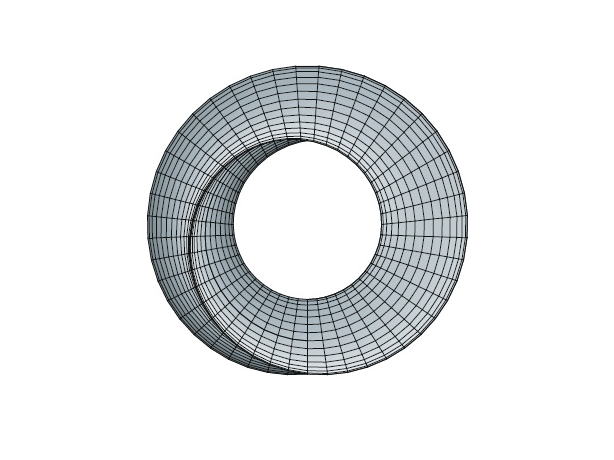
\includegraphics[width=0.7\textwidth]{umblictorus.png}\\[1cm]
 \vfill
 
 
% Bottom of the page
{\large \today}
 
\end{center}
 
\end{titlepage}
%\maketitle
\tableofcontents
\setcounter{chapter}{7}
\chapter{Infinite Series}
\begin{center}
\small{\parbox{18cm}{
		\begin{raggedright}
		{\small
		\textit{A man has one hundred dollars and you leave him with two dollars.  That's subtraction.}
 }
 
				\vspace{.5cm}\hfill{---Mae West}
		\end{raggedright}
	}
} 
\end{center}
One important application of infinite sequences is in representing infinite summations. If $\{a_n\}$ is an infinite sequence, then 
\[\sum _{n=1}^\infty a_n=a_1+a_2+a_3+\cdots \]
is called an \textbf{infinite series} (or simply a \textbf{series}). The numbers $a_1, a_2, a_3, \dots$ are called the \textbf{terms} of the series. To find the sum of an infinite series, consider the following \textbf{sequence of partial sums}.
\begin{eqnarray*}
S_1 &=& a_1\\
S_2 &=& a_1 +a_2 \\
S_3 &=& a_1 +a_2 +a_3 \\
\vdots &=& \vdots \quad \quad  \vdots \quad \quad \vdots \\
S_n &=& a_1 +a_2 +a_3 + \cdots + a_n.
\end{eqnarray*}
If this sequence of partial sums converges, then the series is said to converge and has the sum indicated in the following definition.

\section{Definition of Convergent and Divergent Series}
For the infinite series $\displaystyle \sum a_n$, the \textbf{$n$th partial sum} is given by 
\[S_n=a_1+a_2+a_3+\cdots +a_n.\]
If the sequence of partial sums $\{S_n\}$ converges to $S$, then the series $\displaystyle \sum a_n$ \textbf{converges}. The limit $S$ is called the \textbf{sum of the series}. If $\{S_n\}$ diverges, then the series \textbf{diverges}.
\begin{example}
The series $\displaystyle \sum _{n=1}^\infty \dfrac{1}{2^n}=\dfrac{1}{2}+\dfrac{1}{4}+\dfrac{1}{8}+\dfrac{1}{16}+\cdots$ has the following partial sums.
\begin{eqnarray*}
S_1 &=& \dfrac{1}{2}\\
S_2 &=& \dfrac{1}{2}+\dfrac{1}{4}=\dfrac{3}{4} \\
s_3 &=& \dfrac{1}{2}+\dfrac{1}{4} +\dfrac{1}{8} = \dfrac{7}{8} \\
\vdots &=& \vdots \quad \quad \vdots \quad \quad \vdots \quad \vdots \\
s_n &=& \dfrac{1}{2}+\dfrac{1}{4} +\dfrac{1}{8} +\cdots + \dfrac{1}{2^n} =\dfrac{2^n-1}{2^n}.
\end{eqnarray*}
Because $\displaystyle \lim _{n\rightarrow \infty}\dfrac{2^n-1}{2^n}=1$, it follows that the series converges and its sum is $1$.
\end{example}
\begin{example}\label{groo}
The $n$th partial sum of the series 
\[\sum _{n=1}^\infty \left(\dfrac{1}{n}-\dfrac{1}{n+1}\right)=\left(1-\dfrac{1}{2}\right)+\left(\dfrac{1}{2}-\dfrac{1}{3}\right)+\left(\dfrac{1}{3}-\dfrac{1}{4}\right)+\cdots\] is given by $S_n=1-\dfrac{1}{n+1}$. Because the limit of $S_n$ is $1$, the series converges and its sum is $1$.
\end{example}
\begin{example}
The series $\displaystyle \sum _{n=1}^\infty 1 =1+1+1+\cdots$ diverges, because $S_n=n$ and the sequence of partial sums diverges.
\end{example}
\noindent The series in Example \eqref{groo} is a \textbf{telescoping series}. That is, it is of the form 
\[ (b_1-b_2)+(b_2-b_3)+(b_3-b_4)+(b_4-b_5)+\cdots \]
note that $b_2$ is canceled by the second term, $b_3$ is canceled by the third term and so on. Because the $n$th partial sum of the series is $S_n=b_1-b_{n+1}$, it follows that a telescoping series will only converge if and only if $b_n$ approaches a finite number as $n\rightarrow \infty$. Moreover, if the series converges, then its sum is 
\[S=b_1-\lim _{n\rightarrow \infty} b_{n+1}.\]
\begin{example}
Find the sum of the series $\displaystyle \sum _{n=1}^\infty \dfrac{2}{4n^2-1}$.

\noindent \textbf{Solution:} Using partial fractions, we can write 
\[a_n=\dfrac{2}{4n^2-1}=\dfrac{2}{(2n-1)(2n+1)}=\dfrac{1}{2n-1}-\dfrac{1}{2n+1}.\]
From the telescoping form, we can see that the $n$th partial sum is 
\[S_n=\left(\dfrac{1}{1}-\dfrac{1}{3}\right)+\left(\dfrac{1}{3}-\dfrac{1}{5}\right)+\cdots +\left(\dfrac{1}{2n-1}-\dfrac{1}{2n+1}\right)=1-\dfrac{1}{2n+1}.\] Thus, the series converges and its sum is $1$. That is,
\[\sum _{n=1}^\infty \dfrac{2}{4n^2-1}=\lim _{n\rightarrow \infty} S_n=\lim _{n\rightarrow \infty}\left(1-\dfrac{1}{2n+1}\right)=1.\] 
\end{example}
\section{Geometric Series}
A geometric series with ratio $r$ is given by 
\[\sum _{n=0}^\infty ar^n =a+ar+ar^2+\cdots +ar^n + \cdots , a\neq 0.\]
\begin{theorem}
A geometric series with ratio $r$ diverges if $|r|\geq 1$. If $0<|r|<1$, then the series converges to the sum $\displaystyle \sum _{n=0}^\infty ar^n=\dfrac{a}{1-r}, \quad  0<|r|<1.$
\end{theorem}
\begin{example}
The geometric series 
\[\sum _{n=0}^\infty \dfrac{3}{2^n}=\sum _{n=0}^\infty 3\left(\dfrac{1}{2}\right)^n=3(1)+3\left(\dfrac{1}{2}\right)+3\left(\dfrac{1}{2}\right)^2+\cdots\]
has a ratio of $r=\frac{1}{2}$ with $a=3$. Because $0<|r|<1$, the series converges and its sum is $S=\dfrac{a}{1-r}=\dfrac{3}{1-\frac{1}{2}}=6$.
\end{example}
\subsection{Properties of Infinite Series}
If $\displaystyle \sum a_n =A$ and $\displaystyle \sum b_n=B$ and $c$ is a real number, then the following series converge to the indicated sums. (i)\, $\displaystyle \sum ca_n=cA$ \quad (ii)\, $\displaystyle \sum (a_n\pm b_n)=\sum a_n \pm \sum b_n =
A\pm B$. 
\subsubsection{$n$-th Term Test for Divergence}
\subsubsection{Limit of $n-$th Term of a Convergent Series}
If the series $\displaystyle \sum a_n$ converges, then the sequence $\{a_n\}$ converges to $0$.

\noindent If the sequence $\{a_n\}$ does not converge to $0$, then the series $\displaystyle \sum a_n$ diverges. 
\section{Test for Convergence or Divergence of Series}
In this and the following section, we will study several convergence tests that apply to series with \textbf{positive} terms.
\subsection{The Integral Test}
If $f$ is positive, continuous, and decreasing for $x\geq 1$ and $a_n=f(n)$, then $\displaystyle \sum _{n=1}^\infty a_n$ and $\displaystyle \int _1^\infty f(x)\, dx$ either both converge or both diverge.
\begin{example}
Apply the integral test to the series $\displaystyle \sum _{n=1}^\infty \dfrac{n}{n^2+1}$.

\noindent Because $f(x)=\dfrac{x}{x^2+1}$ satisfies the conditions for the integral test (check this), we can integrate to obtain
\begin{eqnarray*}
\int _1^\infty \dfrac{x}{x^2+1}\, dx &=& \dfrac{1}{2}\int _1^\infty \dfrac{2x}{x^2+1}\, dx =\dfrac{1}{2}\lim _{b\rightarrow \infty} \int _1^b \dfrac{2x}{x^2+1}\, dx \\
&=& \dfrac{1}{2}\lim _{b\rightarrow \infty}\biggl[\ln (x^2+1)\biggr]_1^b\\
&=& \dfrac{1}{2}\lim _{b\rightarrow \infty} [\ln (b^2+1)-\ln 2]\\
&=& \infty .
\end{eqnarray*}
Thus, the series \textit{diverges}.
\end{example}
\begin{example}
Apply the integral test to the series $\displaystyle \sum _{n=1}^\infty \dfrac{1}{n^2+1}$.

\noindent \textbf{Solution:} Because $f(x)=\dfrac{1}{x^2+1}$ satisfies the conditions for the integral test, we can integrate to obtain 
\begin{eqnarray*}
\int _1^\infty \dfrac{dx}{x^2+1} &=& \lim _{b\rightarrow \infty}\int _1^b \dfrac{dx}{x^2+1} = \lim _{b\rightarrow \infty} \biggl[\tan ^{-1} x\biggr]_1^b \\
&=& \lim _{b\rightarrow \infty} (\tan ^{-1} b-\tan ^{-1} 1) \\
&=& \dfrac{\pi}{2}-\dfrac{\pi}{4} =\dfrac{\pi}{4}.
\end{eqnarray*} 
Thus, the series \textit{converges}.
\end{example}
\subsection{$p-$ Series and Harmonic Series}
A series of the form 
\[\sum _{n=1}^\infty \dfrac{1}{n^p}=\dfrac{1}{1^p}+\dfrac{1}{2^p}+\dfrac{1}{3^p}+\cdots\] is a \textbf{$p-$series}, where $p$ is a positive constant. For $p=1$, the series 
\[\sum _{n=1}^\infty \dfrac{1}{n}=1+\dfrac{1}{2}+\dfrac{1}{3}+\cdots\] is the \textbf{harmonic series}.
\begin{theorem}
The $p-$series 
\[\sum _{n=1}^\infty \dfrac{1}{n^p}=\dfrac{1}{1^p}+\dfrac{1}{2^p}+\dfrac{1}{3^p}+\cdots\] (i)\, converges if $p>1$ and (ii)\, diverges if $0<p\leq 1$.
\end{theorem}
\begin{example}
From the Theorem it follows that the harmonic series \[\sum _{n=1}^\infty \dfrac{1}{n}=1+\dfrac{1}{2}+\dfrac{1}{3}+\cdots\] diverges.
\end{example}
\section{Comparisons of Series}
\subsection{Direct Comparison Test}
This is  a test for positive-term series. It allows you to compare a series having complicated terms with a simpler series whose convergence or divergence is known.

\subsubsection{Direct Comparison Test}
\begin{theorem}
Let $0\leq a_n\leq b_n$ for all $n$.
\begin{enumerate}
\item If $\displaystyle \sum _{n=1}^\infty b_n$ converges, then $\displaystyle \sum _{n=1}^\infty a_n$ converges.
\item If $\displaystyle \sum _{n=1}^\infty a_n$ diverges, then $\displaystyle \sum _{n=1}^\infty b_n$ diverges.
\end{enumerate}
\end{theorem}
\begin{example}
Determine the convergence or divergence of $\displaystyle \sum _{n=1}^\infty \dfrac{1}{2+3^n}$.

\noindent \textbf{Solution:} This series resembles $\displaystyle \sum _{n=1}^\infty \dfrac{1}{3^n}$ (Convergent geometric series). Term-by-term comparison yields 
\[a_n=\dfrac{1}{2+3^n}<\dfrac{1}{3^n}=b_n, \quad n\geq 1.\]
Thus, by the Direct Comparison Test, the series converges.
\end{example}
\begin{example}
Determine the convergence or divergence of $\displaystyle \sum _{n=1}^\infty \dfrac{1}{2+\sqrt{n}}$.

\noindent \textbf{Solution:} The series resembles $\displaystyle \sum _{n=1}^\infty \dfrac{1}{n^{\frac{1}{2}}}$ (Divergent $p-$series). Term-by-term comparison yields 
\[\dfrac{1}{2+\sqrt{n}}\leq \dfrac{1}{\sqrt{n}}, \quad n\geq 1\]
which does not meet the requirements for divergence. Still expecting the series to diverge, we can compare the given series with $\displaystyle \sum _{n=1}^\infty \dfrac{1}{n}$ (Divergent Harmonic series). In this case, term-by-term comparison yields 
\[a_n=\dfrac{1}{n}\leq \dfrac{1}{2+\sqrt{n}}=b_n, \quad n\geq 4\] and, by the Direct Comparison Test, the given series diverges.
\end{example}
\subsection{Limit Comparison Test or Quotient Test}
Often a given series closely resembles a $p-$series or a geometric series, yet we cannot establish the term-by-term comparison necessary to apply the Direct Comparison Test. We can apply a second comparison test, called the \textbf{Limit Comparison Test}.

\subsubsection{Limit Comparison Test}
Suppose that $a_n>0$ and $b_n>0$ and $\displaystyle \lim _{n\rightarrow \infty}\left(\dfrac{a_n}{b_n}\right)=L$ where $L$ is finite and positive. Then the two series $\displaystyle \sum a_n$ and $\displaystyle \sum b_n$, either both converge or both diverge. If $L=0$ and $\displaystyle \sum b_n$ converges, then $\displaystyle \sum a_n$ converges. If $L=\infty$ and $\displaystyle \sum b_n$ diverges, then $\displaystyle \sum a_n$ diverges.

\begin{example}
Show that the following harmonic series diverges.
\[\sum _{n=1}^\infty \dfrac{1}{an+b}, \quad a>0, \, b>0.\]

\noindent \textbf{Solution:} By comparison with $\displaystyle \sum _{n=1}^\infty \dfrac{1}{n}$ we have $\displaystyle \lim _{n\rightarrow \infty} \dfrac{\frac{1}{an+b}}{\frac{1}{n}}=\lim _{n\rightarrow \infty}\dfrac{n}{an+b}=\dfrac{1}{a}$. Because this limit is grater than $0$, we can conclude from the Limit comparison Test that the given series diverges.
\end{example}
\noindent The limit Comparison Test works well for comparing a messy algebraic series with a $p-$series. In choosing an appropriate $p-$series, we must choose one with an $n$th term of the same magnitude as the $n$th term of the given series.
\begin{center}
  \begin{tabular}{ l |l |l }
 
    Given series & Comparison series & Conclusion \\ \hline
    $\displaystyle \sum _{n=1}^\infty \dfrac{1}{3n^2-4n+5}$ & $\displaystyle \sum _{n=1}^\infty \dfrac{1}{n^2}$ & Both series converge. \\ \hline
    $\displaystyle \sum _{n=1}^\infty \dfrac{1}{\sqrt{3n-2}}$ & $\displaystyle \sum _{n=1}^\infty \dfrac{1}{\sqrt{n}}$ & Both series diverge. \\
    \hline
    $\displaystyle \sum _{n=1}^\infty \dfrac{n^2-10}{4n^5+n^3}$ & $ \displaystyle \sum _{n=1}^\infty \dfrac{n^2}{n^5}=\sum _{n=1}^\infty \dfrac{1}{n^3}$ & Both series converge.\\ \hline
  \end{tabular}
\end{center}
\section{Alternating Series}
So far, most series we have dealt with have had positive terms. In this section, we will study series that contain both positive and negative terms. The simplest such series is an \textbf{alternating series}, whose terms alternate in sign. For example, the geometric series
\[\sum _{n=0}^\infty \left(-\dfrac{1}{2}\right)^n=\sum _{n=0}^\infty (-1)^n \dfrac{1}{2^n}=1-\dfrac{1}{2}+\dfrac{1}{4}-\dfrac{1}{8}+\dfrac{1}{16}-\cdots \]
is an alternating geometric series with $r=-\frac{1}{2}$. Alternating series occur in two ways, either the odd terms are negative or the even terms are negative.
\subsubsection{Alternating Series Test}
Let $a_n>0$. The alternating series $\displaystyle \sum _{n=1}^\infty (-1)^na_n$ and $\displaystyle \sum _{n=1}^\infty (-1)^{n+1}a_n$ converge, if the following two conditions are met. 
\begin{enumerate}
\item $a_{n+1}\leq a_n$ for all $n$.
\item $\displaystyle \lim _{n\rightarrow \infty} a_n =0$.
\end{enumerate}
\begin{example}
Determine the convergence or divergence of $\displaystyle \sum _{n=1}^\infty (-1)^{n+1}\dfrac{1}{n}$.

\noindent \textbf{Solution:} Because $\dfrac{1}{n+1}\leq \dfrac{1}{n}$ for all $n$ and the limit (as $n\rightarrow \infty$) of $\dfrac{1}{n}$ is $0$, we can apply the Alternating Series Test to conclude that the series converges.  (This series is called the alternating harmonic series)
\end{example} 
\begin{example}
Determine the convergence or divergence of $\displaystyle \sum _{n=1}^\infty \dfrac{n}{(-2)^{n-1}}$.

\noindent \textbf{Solution:} To apply the Alternating Series Test, note that, for $n\geq 1$, 
\begin{eqnarray*}
\dfrac{1}{2}&\leq & \dfrac{n}{n+1}\\
\dfrac{2^{n-1}}{2^n} & \leq & \dfrac{n}{n+1} \\
(n+1)2^{n-1} &\leq & n2^n \\
\dfrac{n+1}{2^n} & \leq & \dfrac{n}{2^{n-1}}.
\end{eqnarray*}
Hence, $a_{n+1}=\dfrac{n+1}{2^{n}}\leq \dfrac{n}{2^{n-1}}=a_n$ for all $n$. Furthermore, by L'Hopital's rule, 
\[\lim_{n\rightarrow \infty}\dfrac{n}{2^{n-1}}=\lim _{n\rightarrow \infty}\dfrac{1}{2^{n-1}(\ln 2)}=0\Longrightarrow \lim _{n\rightarrow \infty} \dfrac{n}{2^{n-1}}=0.\] Therefore, by the Alternating Series Test, the given series converges. 
\end{example}
\subsubsection{Cases for which the Alternating Series Test Fails}
\begin{example}
The alternating series 
\[\sum _{n=1}^\infty \dfrac{(-1)^{n+1}(n+1)}{n}=\dfrac{2}{1}-\dfrac{3}{2}+\dfrac{4}{3}-\dfrac{5}{4}+\dfrac{6}{5}-\cdots\] passes the first condition in the alternating series test because $a_{n+1}\leq a_n$ for all $n$. We cannot apply the Alternating Series Test, because the series does not  pass the second condition.

\noindent The alternating series 
\[\dfrac{2}{1}-\dfrac{1}{1}+\dfrac{2}{2}-\dfrac{1}{2}+\dfrac{2}{3}-\dfrac{1}{3}
+\dfrac{1}{2}-\dfrac{1}{4}+\cdots\] passes the second condition because $a_n$ approaches $0$ as $n\rightarrow \infty$. We cannot apply the Alternating Series Test, however, because the series does not pass the first condition.
\end{example}
\section{Absolute and Conditional Convergence}
Occasionally, a series may have both positive and negative terms and not be an alternating series, for example, the series 
\[\sum _{n=1}^\infty \dfrac{\sin n}{n^2}=\dfrac{\sin 1}{1}+\dfrac{\sin 2}{4}+\dfrac{\sin 3}{9}+\cdots\] has both positive and negative terms, yet it is not an alternating series. One way to obtain some information about the convergence of this series is to investigate the convergence of the series $\displaystyle \sum _{n=1}^\infty \left|\dfrac{\sin n}{n^2}\right|$. By direct comparison, we have $|\sin n|\leq 1$, for all $n$, so 
\[\left|\dfrac{\sin n}{n^2}\right| \leq \dfrac{1}{n^2}, \quad n\geq 1.\]
Thus, by the Direct Comparison Test, the series $\displaystyle \sum _{n=1}^\infty \dfrac{\sin n}{n^2}$ converges. But the question still is ``Does the original series converge?'' 
\begin{theorem}[Absolute Convergence]
If the series $\displaystyle \sum |a_n|$ converges, then the series $\displaystyle \sum a_n$ also converges.
\end{theorem}
\noindent The converse of the Theorem is not true. For example, the alternating harmonic series 
\[ \sum _{n=1}^\infty \dfrac{(-1)^{n+1}}{n}=1-\dfrac{1}{2}+\dfrac{1}{3}-\dfrac{1}{4}+\cdots\] converges by the Alternating Series Test. Yet the harmonic series diverges. This type of convergence is called \textbf{conditional}.
\subsubsection{Definition of Absolute and Conditional Convergence}
\begin{enumerate}
\item $\displaystyle \sum a_n$ is \textbf{absolutely convergent} if $\displaystyle \sum |a_n|$ converges.
\item $\displaystyle \sum a_n$ is \textbf{conditionally convergent } if $\displaystyle \sum a_n$ converges but $\displaystyle \sum |a_n|$ diverges.
\item An absolutely convergent series converges.
\end{enumerate}
\begin{example}
Determine whether the following series are convergent or divergent. Classify any convergent  series as absolutely or conditionally convergent.\\
(a)\, $\displaystyle \sum _{n=1}^\infty \dfrac{(-1)^{\frac{n(n+1)}{2}}}{3^n}=-\dfrac{1}{3}-\dfrac{1}{9}+\dfrac{1}{27}+\dfrac{1}{81}-\cdots$.

\noindent \textbf{Solution:} This in not an alternating series. However, because
\[\sum _{n=1}^\infty \left |\dfrac{(-1)^{\frac{n(n+1)}{2}}}{3^n}\right|=\sum _{n=1}^\infty \dfrac{1}{3^n}\] is a convergent geometric series, so the given series is absolutely convergent, hence convergent.

\noindent (b)\, $\displaystyle \sum _{n=1}^\infty \dfrac{(-1)^n}{\ln (n+1)}=-\dfrac{1}{\ln 2}+\dfrac{1}{\ln 3}-\dfrac{1}{\ln 4}+\dfrac{1}{\ln 5}-\cdots$.

\noindent \textbf{Solution:} In this case, the alternating series test indicates that the given series converges. However, the series 
\[\sum _{n=1}^\infty \left|\dfrac{(-1)^n}{\ln (n+1)}\right|=\dfrac{1}{\ln 2}+\dfrac{1}{\ln 3}+\dfrac{1}{\ln 4}+\cdots\] diverges by direct comparison with terms of the harmonic series. Therefore, the given series is conditionally convergent.

\noindent (c)\, $\displaystyle \sum _{n=1}^\infty \dfrac{(-1)^n}{\sqrt{n}}=-\dfrac{1}{\sqrt{1}}+\dfrac{1}{\sqrt{2}}-\dfrac{1}{\sqrt{3}}+\dfrac{1}{\sqrt{4}}-\cdots$.

\noindent \textbf{Solution:} The given series converges by the Alternating Series Test. Moreover, because the $p-$series 
\[\sum _{n=1}^\infty \left|\dfrac{(-1)^n}{\sqrt{n}}\right|=\dfrac{1}{\sqrt{1}}+\dfrac{1}{\sqrt{2}}+\dfrac{1}{\sqrt{3}}+\dfrac{1}{\sqrt{4}}+\cdots\] diverges, the given series is conditionally convergent.
\end{example}
\section{The Ratio and Root Tests}
\subsection{The Ratio Test}
This is a test for absolute convergence.
\subsubsection{Ratio Test}
\begin{enumerate}
\item $\displaystyle \sum a_n$ converges absolutely if $\displaystyle \lim _{n\rightarrow \infty}\left|\dfrac{a_{n+1}}{a_n}\right|<1$.
\item $\displaystyle \sum a_n$ diverges if $\displaystyle \lim _{n\rightarrow \infty}\left|\dfrac{a_{n+1}}{a_n}\right|>1$ or $\displaystyle \lim _{n\rightarrow \infty}\left|\dfrac{a_{n+1}}{a_n}\right|=\infty$.
\item The Ratio Test is inconclusive if $\displaystyle \lim _{n\rightarrow \infty}\left|\dfrac{a_{n+1}}{a_n}\right|=1$.
\end{enumerate}
Although the Ratio Test is not a cure for all ills related to tests for convergence, it is particularly useful for series that \textit{converge rapidly}. Series involving factorials or exponentials are frequently of this type. 
\begin{example}
Determine the convergence or divergence of $\displaystyle \sum _{n=0}^\infty \dfrac{2^n}{n!}$.

\noindent \textbf{Solution:} Because $a_n=\dfrac{2^n}{n!}$, we can write the following 
\begin{eqnarray*}
\lim _{n\rightarrow \infty}\left|\dfrac{a_{n+1}}{a_n}\right| &=& \lim _{n\rightarrow \infty} \left[\dfrac{2^{n+1}}{(n+1)!}\div \dfrac{2^n}{n!}\right]\\
&=& \lim _{n\rightarrow \infty} \left[\dfrac{2^{n+1}}{(n+1)!}\cdot \dfrac{n!}{2^n}\right]\\
&=& \lim _{n\rightarrow \infty} \dfrac{2}{n+1} \\
&=& 0.
\end{eqnarray*}
Therefore, the series converges.
\end{example}
\begin{example}
Determine whether the following series converge or diverge.\\
(a)\, $\displaystyle \sum _{n=0}^\infty \dfrac{n^22^{n+1}}{3^n}$ \quad (b)\, $\displaystyle \sum _{n=1}^\infty \dfrac{n^n}{ n!}$.

\noindent \textbf{Solution:} \\
(a)\, This series converges because the limit of $\left|\dfrac{a_{n+1}}{a_n}\right|$ is less than $1$.
\begin{eqnarray*}
\lim _{n\rightarrow \infty} \left|\dfrac{a_{n+1}}{a_n}\right| &=& \lim _{n\rightarrow \infty} \left[ (n+1)^2\left(\dfrac{2^{n+2}}{3^{n+1}}\right)\left(\dfrac{3^n}{n^22^{n+1}}\right)\right] \\
&=& \lim _{n\rightarrow \infty} \dfrac{2(n+1)^2}{3n^2}\\
&=& \dfrac{2}{3} <1.
\end{eqnarray*}
\noindent (b)\, This series diverges because the limit of $\left|\dfrac{a_{n+1}}{a_n}\right|$ is grater than $1$.
\begin{eqnarray*}
\lim _{n\rightarrow \infty} \left|\dfrac{a_{n+1}}{a_n}\right| &=& \lim _{n\rightarrow \infty}\left[\dfrac{(n+1)^{n+1}}{(n+1)!}\left(\dfrac{n!}{n^n}\right)\right] \\
&=& \lim _{n\rightarrow \infty} \left[\dfrac{(n+1)^{n+1}}{(n+1)}\left(\dfrac{1}{n^n}\right)\right]\\
&=& \lim _{n\rightarrow \infty} \dfrac{(n+1)^n}{n^n} =\lim _{n\rightarrow \infty} \left(1+\dfrac{1}{n}\right)^n\\
&=& e >1. 
\end{eqnarray*}
\end{example}
\subsection{The Root Test}
This test of convergence or divergence of series works especially well for series involving $n$th powers.
\subsubsection{Root Test}
Let $\displaystyle \sum a_n$ be a series with non-zero terms.
\begin{enumerate}
\item $\displaystyle \sum a_n$ converges absolutely if $\displaystyle \lim _{n\rightarrow \infty} \sqrt[n]{|a_n|}<1$.
\item $\displaystyle \sum a_n$ diverges if $\displaystyle \lim _{n\rightarrow \infty} \sqrt[n]{|a_n|}>1$ or $\displaystyle \lim _{n\rightarrow \infty} \sqrt[n]{|a_n|}=\infty$.
\item The Root Test is inconclusive if $\displaystyle \lim _{n\rightarrow \infty} \sqrt[n]{|a_n|}=1$. 
\end{enumerate}
\begin{example}
Determine the convergence or divergence of $\displaystyle \sum _{n=1}^\infty \dfrac{e^{2n}}{n^n}$.

\noindent \textbf{Solution:} We can apply the Root Test as follows 
\begin{eqnarray*}
\lim _{n\rightarrow \infty} \sqrt[n]{|a_n|} &=& \lim _{n\rightarrow \infty} \sqrt[n]{\dfrac{e^{2n}}{n^n}}\\
&=& \lim _{n\rightarrow \infty} \dfrac{e^{\frac{2n}{n}}}{n^{\frac{n}{n}}}\\
&=& \lim _{n\rightarrow \infty} \dfrac{e^2}{n}\\
&=& 0<1.
\end{eqnarray*} 
Because this limit is less than $1$, we can conclude that the series converges absolutely.
\end{example}
\section{Power Series}
\subsection{Definition of Power Series}
If $x$ is a variable, then the infinite series of the form 
\[\sum _{n=0}^\infty a_nx^x=a_0+a_1x+a_2x^2+a_3x^3+\cdots + a_nx^n+\cdots\] is called a \textbf{power series}. More generally, a series of the form 
\[\sum _{n=0}^\infty a_n(x-c)^n=a_0+a_1(x-c)+a_2(x-c)^2+\cdots +a_n(x-c)^n +\cdots\] is called a \textbf{power series centered at c}, where $c$ is a constant.
\begin{example}
(a)\, The following power series is centered at $0$.
\[\sum _{n=0}^\infty \dfrac{x^n}{n!}=1+x+\dfrac{x^2}{2}+\dfrac{x^3}{3!}+\cdots\]\\
(b)\, The following power series is centered at $-1$.
\[\sum _{n=0}^\infty (-1)^n(x+1)^n=1-(x+1)+(x+1)^2-(x+1)^3+\cdots\]
(c)\, The following power series is centered at $1$.
\[\sum _{n=1}^\infty \dfrac{1}{n}(x-1)^n=(x-1)+\dfrac{1}{2}(x-1)^2+\dfrac{1}{3}(x-1)^3+\cdots \]
\end{example}
\subsection{Radius and Interval of Convergence}
A power series in $x$ can be viewed as a function of $x$
\[f(x)=\sum _{n=0}^\infty a_n(x-c)^n\] where the \textit{domain of f} is the set of all $x$ for which the power series converges.

\subsubsection{Convergence of a Power Series}
For a power series centered at $c$, precisely one of the following is true.
\begin{enumerate}
\item The series converges only at $c$.
\item There exists a real number $R>0$ such that the series converges absolutely for $|x-c|<R$, and diverges for $|x-c|>R$.
\item The series converges absolutely for all $x$.
\end{enumerate}
The number $R$ is the \textbf{radius of convergence} of the power series. In the series converges only at $c$, then the radius of convergence is $R=0$, and if the series converges for all $x$, then the radius of convergence is $R=\infty$. The set of all values of $x$ for which the power series converges is the \textbf{interval of convergence} of the power series. 
\begin{example}
Find the radius of convergence of $\displaystyle \sum _{n=0}^\infty n!x^n$.

\noindent \textbf{Solution:} For $x=0$, we obtain 
\[f(0)=\sum _{n=0}^\infty n!0^n=1+0+0+\cdots =1.\] For any fixed value of $x$ such that $|x|>0$, let $u_n=n!x^n$. Then 
\begin{eqnarray*}
\lim _{n\rightarrow \infty} \left|\dfrac{u_{n+1}}{u_n}\right| &=& \lim _{n\rightarrow \infty}\left|\dfrac{(n+1)!x^{n+1}}{n!x^n}\right|\\
&=& |x| \lim _{n\rightarrow \infty} (n+1)\\
&=& \infty .
\end{eqnarray*}
Therefore, by the Ratio Test, the series diverges for $|x|>0$, and converges only at its center, $0$. Hence, the radius of convergence is $R=0$.
\end{example}
\begin{example}
Find the radius of convergence of $\displaystyle \sum _{n=0}^\infty 3(x-2)^n$.

\noindent \textbf{Solution:} For $x\neq 2$, let $u_n=3(x-2)^n$. Then 
\begin{eqnarray*}
\lim _{n\rightarrow \infty} \left|\dfrac{u_{n+1}}{u_n}\right| &=& \lim _{n\rightarrow \infty}\left|\dfrac{3(x-2)^{n+1}}{3(x-2)^n}\right|\\
&=& \lim _{n\rightarrow \infty} |x-2|\\
&=&|x-2|.
\end{eqnarray*}
By the Ratio Test, the series converges if $|x-2|<1$ and diverges if $|x-2|>1$. Therefore, the radius of convergence of the series is $R=1$. 
\end{example}
\subsubsection{Finding the Interval of Convergence}
\begin{example}
Find the interval of convergence of $\displaystyle \sum _{n=1}^\infty \dfrac{x^n}{n}$.

\noindent \textbf{Solution:} Letting $u_n=\dfrac{x^n}{n}$ produces 
\begin{eqnarray*}
\lim _{n\rightarrow \infty} \left|\dfrac{u_{n+1}}{u_n}\right| &=& \lim _{n\rightarrow \infty}\left|\dfrac{\frac{x^{n+1}}{n+1}}{\frac{x^n}{n}}\right|\\
&=& \lim _{n\rightarrow \infty} \left|\dfrac{nx}{n+1}\right|\\
&=& |x|.
\end{eqnarray*}
Therefore, by the Ratio Test, the radius of convergence is $R=1$. Moreover, because the series is centered at $0$, it converges in the interval $(-1,1)$. This interval, however, is not necessarily the interval of convergence. To determine this, we must test for convergence at each endpoint. When $x=1$, we obtain the divergent harmonic series 
\[\sum _{n=1}^\infty \dfrac{ 1}{n}=1+\dfrac{1}{2}+\dfrac{1}{3}+\cdots\] When $x=-1$, we obtain the convergent alternating harmonic series \[\sum _{n=1}^\infty \dfrac{(-1)^n}{n}=-1+\dfrac{1}{2}-\dfrac{1}{3}+\dfrac{1}{4}-\cdots\] Therefore, the interval of convergence for the series is $[-1,1)$.
\end{example}
\begin{example}
Find the interval of convergence of $\displaystyle \sum _{n=0}^\infty \dfrac{(-1)^n(x+1)^n}{2^n}$.

\noindent \textbf{Solution:} Letting $u_n=\dfrac{(-1)^n(x+1)^n}{2^n}$ produces 
\begin{eqnarray*}
\lim _{n\rightarrow \infty} \left|\dfrac{u_{n+1}}{u_n}\right| &=& \lim _{n\rightarrow \infty}\left|\dfrac{\frac{(-1)^{n+1}(x+1)^{n+1}}{2^{n+1}}}{\frac{(-1)^n(x+1)^n}{2^n}}\right|\\
&=& \lim _{n\rightarrow \infty} \left|\dfrac{2^n(x+1)}{2^{n+1}}\right|\\
&=& \left|\dfrac{x+1}{2}\right|.
\end{eqnarray*}
By the Ratio test, the series converges if $\left|\dfrac{x+1}{2}\right| <1$ or $|x+1|<2$. Hence, the radius of convergence is $R=2$. Because the series is centered at $x=-1$, it will converge in the interval $(-3,1)$. Furthermore, at the endpoints we have 
\[\sum _{n=0}^\infty \dfrac{(-1)^n(-2)^n}{2^n}=\sum _{n=0}^\infty \dfrac{2^n}{2^n}=\sum _{n=0}^\infty 1 \quad (\mbox{Diverges when x=-3})\] and \[\sum _{n=0}^\infty \dfrac{(-1)^n(2)^n}{2^n}=\sum _{n=0}^\infty (-1)^n \quad (\mbox{Diverges when  x=1})\]
both of which diverge. Thus, the interval of convergence is $(-3,1)$.
\end{example}
\begin{example}
Find the interval of convergence of $\displaystyle \sum _{n=1}^\infty \dfrac{x^n}{n^2}$.

\noindent \textbf{Solution:} Letting $u_n=\dfrac{x^n}{n^2}$ produces 
\begin{equation*}
\lim _{n\rightarrow \infty} \left|\dfrac{u_{n+1}}{u_n}\right| = \lim _{n\rightarrow \infty}\left|\dfrac{\frac{x^{n+1}}{(n+1)^2}}{\frac{x^n}{n^2}}\right| =\lim _{n\rightarrow \infty} \left| \dfrac{n^2x}{(n+1)^2}\right| =|x|.
\end{equation*}
Thus, the radius of convergence is $R=1$. Because the series is centered at $x=0$, it converges in the interval $(-1,1)$. When  $x=1$, we obtain the convergent $p-$series \[\sum _{n=1}^\infty \dfrac{1}{n^2}=1+\dfrac{1}{2^2} +\dfrac{1}{3^2}+\dfrac{1}{4^2}+\cdots \quad (\mbox{Converges when x=1})\]
When $x=-1$, we obtain the convergent alternating series 
\[\sum _{n=1}^\infty \dfrac{(-1)^n}{n^2}=-1+\dfrac{1}{2^2}-\dfrac{1}{3^2}+\dfrac{1}{4^2}-\cdots \quad (\mbox{Converges when x=-1})\]
Therefore, the interval of convergence for the given series is $[-1,1]$.
\end{example}
\begin{example}
Find the interval of convergence of $\displaystyle \sum _{n=1}^\infty nx^n$.

\noindent \textbf{Solution:} The series is a power series with $a_n=n$ and $c=0$. Let $u_n=nx^n$, so $u_{n+1}=(n+1)x^{n+1}$. Then 
\[\dfrac{u_{n+1}}{u_n}=\dfrac{(n+1)|x|^{n+1}}{n|x|^n}=\dfrac{n+1}{n}|x|\Longrightarrow |x| \quad \mbox{as} \quad n\rightarrow \infty.\]
The limit is less than one whenever $|x|<1$. The Ratio Test then shows $\displaystyle \sum _{n=1}^\infty u_n$ is convergent for $|x|<1$, and the series diverges for $|x|>1$. This means the radius of convergence is $R=1$. We know that the series is convergent for $-1<x<1$. We need to check convergence at the endpoints of this interval. When $x=1$, we have $\displaystyle \sum _{n=1}^\infty n$. This series does not approach zero as $n\rightarrow \infty$, we know this series must diverge. Similarly, the series is divergent when $x=-1$. The interval of convergence is $(-1,1)$.
\end{example}
\begin{example}
Find the interval of convergence of $\displaystyle \sum _{n=1}^\infty \dfrac{(-1)^n(x-2)^n}{n4^n}$.

\noindent \textbf{Solution:} Let $u_n=\dfrac{|x-2|^n}{n4^n}$, so $u_{n+1}=\dfrac{|x-2|^{n+1}}{(n+1)4^{n+1}}$. Then 
\[\dfrac{u_{n+1}}{u_n}=\dfrac{|x-2|^{n+1}}{(n+1)4^{n+1}}\dfrac{n4^n}{|x-2|^n}=\dfrac{n|x-2|}{(n+1)4}\Longrightarrow \dfrac{|x-2|}{4}\quad \mbox{as} \quad n\rightarrow \infty.\]
The Ratio Test gives convergence for $\dfrac{|x-2|}{4}<1$ and divergence for $\dfrac{|x-2|}{4}>1$. Solving the first inequality, we have 
\[|x-2|<4\Longrightarrow -4<x-2<4\Longrightarrow -2<x<6.\]
When $x=-2$, the series is 
\[\sum _{n=1}^\infty \dfrac{(-1)^n(-2-2)^n}{n4^n}=\sum _{n=1}^\infty \dfrac{1}{n},\]
which is a divergent $p-$series. When $x=6$, we have 
\[\sum _{n=1}^\infty \dfrac{(-1)^n(6-2)^n}{n4^n}=\sum _{n=1}^\infty \dfrac{(-1)^n}{n}.\] The Alternating Series Test shows that the series is convergent. The interval of convergence is $-2<x\leq 6$.
\end{example}
\begin{example}
Find the interval of convergence of the series $\displaystyle \sum _{n=1}^\infty \dfrac{x^n}{n3^n}$.

\noindent \textbf{Solution:} With $u_n=\dfrac{x^n}{n3^n}$, we find that 
\[\lim _{n\rightarrow \infty }\left|\dfrac{u_{n+1}}{u_n}\right|=\left|\dfrac{\dfrac{x^{n+1}}{(n+1)3^{n+1}}}{\dfrac{x^n}{n3^n}}\right|=\lim _{n\rightarrow \infty}\dfrac{n|x|}{3(n+1)}=\dfrac{|x|}{3}.\]
Now $\dfrac{|x|}{3}<1$ provided $|x|<3$, so the Ratio Test implies that the given series converges absolutely if $|x|<3$ and diverges if $|x|>3$. When $x=3$, we have the divergent harmonic series $\displaystyle \sum \dfrac{1}{n}$ and when $x=-3$, we have the convergent alternating series $\displaystyle \sum \dfrac{(-1)^n}{n}$. Thus the interval of convergence of the given power series is $[-3,3)$.
\end{example}
\begin{example}
Find the interval of convergence of $\displaystyle \sum _{n=0}^\infty \dfrac{2^nx^n}{n!}$.

\noindent \textbf{Solution:} With $u_n=\dfrac{2^nx^n}{n!}$, we find that 
\[\lim _{n\rightarrow \infty}\left|\dfrac{\dfrac{2^{n+1}x^{n+1}}{(n+1)!}}{\dfrac{2^nx^n}{n!}}\right|=\lim _{n\rightarrow \infty}\dfrac{2|x|}{n+1}=0\] for all $x$. Hence the Ratio Test implies that the power series converges for all $x$, and its interval of convergence is $(-\infty, \infty)$. 
\end{example}
\section{Tutorial Questions}
\begin{enumerate}
\item Find the sum of the convergent series.\\
(i)\, $\displaystyle \sum _{n=0}^\infty \left(\dfrac{1}{2}\right)^n$ \quad (ii)\, $\displaystyle \sum _{n=0}^\infty 2\left(\dfrac{2}{3}\right)^n$ \quad (iii)\, $\displaystyle \sum _{n=0}^\infty \left(\dfrac{-1}{2}\right)^n$ \quad (iv)\, $\displaystyle \sum _{n=2}^\infty \dfrac{1}{n^2-1}$ \quad (v)\, $\displaystyle \sum _{n=1}^\infty \dfrac{1}{n(n+1)}$\\
(vi)\, $\displaystyle \sum _{n=1}^\infty \dfrac{4}{n(n+2)}$ \quad (vii)\, $\displaystyle \sum _{n=1}^\infty \dfrac{1}{(2n+1)(2n+3)}$ \quad (viii)\, $\displaystyle \sum _{n=0}^\infty \left(\dfrac{1}{2^n}-\dfrac{1}{3^n}\right)$.
\item Determine whether or not the series converges and find its sum if it converges\\
(i)\, $\displaystyle \sum _{r=1}^\infty \dfrac{1}{(3r-1)(3r+2)}$ \quad (ii)\, $\displaystyle \sum _{r=1}^\infty \dfrac{1}{(5r-2)(5r+3)}$ \quad (iii)\,$\displaystyle \sum _{r=1}^\infty \dfrac{20}{(7r-3)(7r+4)}$.
\item Use the integral test to determine the convergence or divergence of the series.\\
(i)\, $\displaystyle \sum _{n=1}^\infty \dfrac{1}{n+1}$  \quad (ii)\,  $\displaystyle \sum _{n=1}^\infty ne^{-n}$ \quad (iii)\,  $\displaystyle \sum _{n=1}^\infty \dfrac{1}{4n+1}$ \quad (iv)\,  $\displaystyle \sum _{n=1}^\infty \dfrac{1}{n^3}$ \quad (v)\,  $\displaystyle \sum _{n=1}^\infty \dfrac{1}{n^{\frac{1}{3}}}$.
\item Show that $\displaystyle \sum _{n=2}^\infty \dfrac{1}{n^{1.1}}$ converges and $\displaystyle \sum _{n=2}^\infty \dfrac{1}{n\ln n}$ diverges.
\item Use the Direct Comparison Test to determine the convergence or divergence of the series.\\
(i)\, $\displaystyle \sum _{n=1}^\infty \dfrac{1}{n^2+1}$ \quad (ii)\, $\displaystyle \sum _{n=2}^\infty \dfrac{1}{n-1}$ \quad (iii)\, $\displaystyle \sum _{n=0}^\infty \dfrac{1}{n!}$ \quad (iv)\, $\displaystyle \sum _{n=1}^\infty \dfrac{1}{n^2+1}$ \quad (v)\, $\displaystyle \sum _{n=0}^\infty \dfrac{2^n}{3^n+5}$ \quad (vi)\, $\displaystyle \sum_{n=1}^{\infty} \dfrac{\sin n +\frac{1}{2}}{n(\mbox{In}~n)^2}$.
\item Use the Limit Comparison to determine the convergence or divergence of the series.\\
(i)\, $\displaystyle \sum _{n=1}^\infty \dfrac{n}{n^2+1}$ \quad (ii)\,$\displaystyle \sum _{n=1}^\infty \dfrac{2n^2-1}{3n^5+2n+1}$ \quad (iii)\, $\displaystyle \sum _{n=1}^\infty \dfrac{1}{n\sqrt{n^2+1}}$  \quad (iv)\, $\displaystyle \sum _{n=1}^\infty \dfrac{n+3}{n(n+2)}$ \quad (v)\, $\displaystyle \sum _{n=1}^\infty \dfrac{n}{(n+1)2^{n-1}}$.
\item Use the Alternating Series Test to determine the convergence or divergence of the series.\\
(i)\, $\displaystyle \sum _{n=1}^\infty \dfrac{(-1)^{n+1}}{n}$ \quad (ii)\, $\displaystyle \sum _{n=1}^\infty \dfrac{(-1)^{n+1}n}{2n-1}$ \quad (iii)\, $\displaystyle \sum _{n=2}^\infty \dfrac{(-1)^{n}}{\ln n}$ \quad (iv)\, $\displaystyle \sum _{n=1}^\infty \dfrac{(-1)^{n+1}(n+1)}{\ln (n+1)}$ \quad (v)\, $\displaystyle \sum _{n=1}^\infty \dfrac{(-1)^{n+1}n^3}{n^3+6}$\\
(vi)\, $\displaystyle \sum _{n=0}^\infty \dfrac{(-1)^{n}}{n!}$ \quad (vii)\, $\displaystyle \sum _{n=1}^\infty \dfrac{(-1)^{n+1}\sqrt{n}}{n+2}$ \quad (viii)\, $\displaystyle \sum _{n=1}^\infty \dfrac{(-1)^{n+1}\sqrt{n}}{\sqrt[3]{n}}$ \quad (ix)\, $\displaystyle \sum _{n=1}^\infty \dfrac{1}{n}\cos n\pi$.
\item Determine whether the series converges conditionally or absolutely, or diverges.\\
(i)\, $\displaystyle \sum _{n=1}^\infty \dfrac{(-1)^{n+1}}{(n+1)^2}$ \quad (ii)\, $\displaystyle \sum _{n=1}^\infty \dfrac{(-1)^{n+1}}{n\sqrt{n}}$ \quad (iii)\, $\displaystyle \sum _{n=1}^\infty \dfrac{(-1)^{n+1}(2n+3)}{n+10}$ \quad (iv)\, $\displaystyle \sum _{n=1}^\infty \dfrac{(-1)^{n+1}}{n^{1.5}}$ \\ (v)\, $\displaystyle \sum _{n=1}^\infty \dfrac{(-1)^{n}}{\sqrt[3]{n+1}}$ \quad (vi)\, $\displaystyle \sum _{n=0}^\infty \dfrac{\cos n\pi}{n+1}$ \quad (vii)\, $\displaystyle \sum _{n=0}^\infty \dfrac{(-1)^{n}}{(2n+1)!}$ \quad (viii)\, $\displaystyle \sum _{n=2}^\infty \dfrac{(-1)^{n}n}{n^3-1}$ \quad (ix)\, $\displaystyle \sum _{n=0}^\infty (-1)^ne^{-n^2}$.
\item Use the Ratio Test to test for convergence or divergence of the series.\\
(i)\, $\displaystyle \sum _{n=0}^\infty \dfrac{n!}{3^n}$ \quad (ii)\,  $\displaystyle \sum _{n=1}^\infty \dfrac{n^2}{2^n}$ \quad (iii)\,  $\displaystyle \sum _{n=1}^\infty \dfrac{(-1)^{n-1}\left(\dfrac{3}{2}\right)^n}{n^2}$ \quad (iv)\,  $\displaystyle \sum _{n=0}^\infty \dfrac{(n!)^2}{(3n)!}$ \quad (v)\,  $\displaystyle \sum _{n=0}^\infty \dfrac{4^n}{3^n+1}$.
\item Use the Root Test to test for convergence or divergence of the series.\\
(i)\,  $\displaystyle \sum _{n=1}^\infty \left(\dfrac{n}{2n+1}\right)^n$ \quad (ii)\,  $\displaystyle \sum _{n=2}^\infty \dfrac{(-1)^n}{(\ln n)^n}$ \quad (iii)\,  $\displaystyle \sum _{n=0}^\infty e^{-n}$ \quad (iv)\,  $\displaystyle \sum _{n=1}^\infty  (2\sqrt[n]{n}+1)^n$ \quad (v)\,  $\displaystyle \sum _{n=1}^\infty \left( \dfrac{-2n}{3^n+1}\right)^{3n}$.
\item Show that the series $\displaystyle \sum _{n=1}^\infty \dfrac{r^n}{n!}$ and $\displaystyle \sum _{n=1}^\infty \dfrac{r^n}{n^n}$ are convergent for all $n$ and that $\displaystyle \sum _{n=1}^\infty n!r^n$ and $\displaystyle \sum _{n=1}^\infty n^n r^n$ are convergent for no $r$ except for $r=0$.
\item Show that the series $\displaystyle \sum _{n=1}^\infty \left(\dfrac{nr}{n+1}\right)^n$ and $\displaystyle \sum _{n=1}^\infty \dfrac{n+1}{n^{n+1}}$ are convergent for $r<1$ and divergent for $r\geq 1$.
\item Find the radius of convergence of the power series.\\
(i)\, $\displaystyle \sum _{n=0}^\infty (-1)^n \dfrac{x^n}{n+1} $ \quad (ii)\, $\displaystyle \sum _{n=0}^\infty \dfrac{(2x)^n}{n!} $ \quad (iii)\, $\displaystyle \sum _{n=0}^\infty  \dfrac{(-1)^n x^n}{2^n} $ \quad (iv)\,  $\displaystyle \sum _{n=0}^\infty (4x)^n $.
\item Find the interval of convergence of the power series.\\
(i)\, $\displaystyle \sum _{n=1}^\infty \dfrac{(-1)^nx^n}{n} $ \quad (ii)\, $\displaystyle \sum _{n=1}^\infty \dfrac{(-1)^{n+1}(x-5)^n}{n5^n} $ \quad (iii)\, $\displaystyle \sum _{n=1}^\infty \dfrac{(-1)^{n+1}x^{2n-1}}{2n-1} $ \quad (iv)\, $\displaystyle \sum _{n=0}^\infty \dfrac{(-1)^n(x-4)^nn!}{3^n} $\\
(v)\, $\displaystyle \sum _{n=0}^\infty \dfrac{x^{2n+1}}{(2n+1)!} $ \quad (vi)\, $\displaystyle \sum _{n=0}^\infty \dfrac{(-1)^nx^n}{(n+1)(n+2)} $ \quad (vii)\, $\displaystyle \sum _{n=1}^\infty \dfrac{n!x^n}{(2n)!} $ \quad (viii)\, $\displaystyle \sum _{n=1}^\infty \dfrac{(-1)^{n+1}x^n}{4^n} $.
\end{enumerate}
\end{document}
\end{document}